\subsection{Calculating Vertical Velocities}

\subsubsection{Grid Velocity}
The vertical grid moves as a consequence of using a $\sigma$--coordinate system. The grid velocity is
\begin{equation}
  \label{kin.eq.grid_velo}
  w^{\text{grid}}(\sigma)=\frac{\pd s}{\pd t}+\vec u\cdot\vec\nabla s-\sigma\left(\frac{\pd H}{\pd t}+\vec u\cdot\vec\nabla H\right)
\end{equation}
The numerical implementation of Equation \eqref{kin.eq.grid_velo} is straightforward.

\subsubsection{Vertical Velocity}
The discretised version of the vertical velocity equation \eqref{kin.eq.vert_velo_scaled} is slightly more compilicated because the horizontal velocities are calculated on the $(r,s)$ grid. The vertical velocity at the ice base is $w_{i,j,N}=w^{\text{grid}}_{i,j,N}-B_b{i,j}$, where $B_b{i,j}$ is the basal melt rate. Integrating from the bottom, the vertical velocity is then
\begin{equation}
  \label{kin.eq.wvel_unc}
  \begin{split}
  w_{i,j,k}=-\sum_{\tilde{k}=N-1}^1\left\{\mathcal{H}_{i,j}\left(\frac{u^x_{i,j,k}+u^x_{i,j,k+1}}{2}+\frac{v^y_{i,j,k}+v^y_{i,j,k+1}}{2}\right)(\sigma_{k+1}-\sigma_k)\right. \\
     +(\tilde{u}_{i,j,k+1}-\tilde{u}_{i,j,k})  \left(\tilde{s}^x_{i,j}-\frac12(\sigma_{k+1}+\sigma_k)\tilde{H}^x_{i,j}\right)  \\
     \left.+(\tilde{v}_{i,j,k+1}-\tilde{v}_{i,j,k})  \left(\tilde{s}^y_{i,j}-\frac12(\sigma_{k+1}+\sigma_k)\tilde{H}^y_{i,j}\right)\right\} + w_{i,j,N}
  \end{split}
\end{equation}
with the weighted ice thickness
\begin{equation*}
  \begin{split}
  \mathcal{H}_{i,j}=\frac{4H_{i,j}+2(H_{i-1,j}+H_{i+1,j}+H_{i,j-1}+H_{i,j+1})}{16}\\
  +\frac{H_{i-1,j-1}+H_{i+1,j-1}+H_{i+1,j+1}+H_{i-1,j+1}}{16}    
  \end{split}
\end{equation*}

This scheme produces vertical velocities at the ice divide which are too small. The vertical velocities on the ice surface are given by the upper kinematic boundary condition, Equation \eqref{kin.eq.upper_bc}. Equation \eqref{kin.eq.wvel_unc} can be corrected with:
\begin{equation}
  \label{kin.eq.wvel_cor}
   w^\ast_{i,j,k}=w_{i,j,k}-(1-\sigma_k)(w_{i,j,k}-{w_s}_{i,j}),
\end{equation}
where ${w_s}_{i,j}$ is the vertical velocity at the ice surface given by \eqref{kin.eq.upper_bc}. Figure \ref{kin.fig.w_profile} shows the different vertical velocities at the ice surface.
\begin{figure}[htbp]
  \centering
  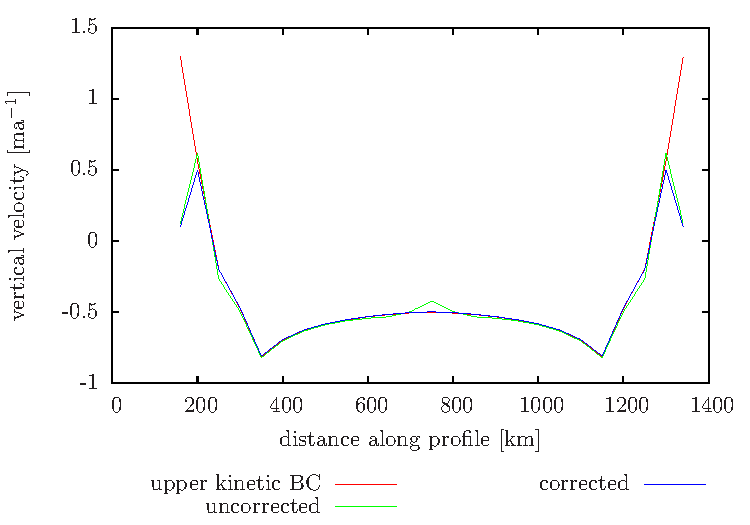
\includegraphics{\dir/gnu/w_profile.eps}
  \caption{Vertical ice surface velocities of the EISMINT-1 moving margin experiment.}
  \label{kin.fig.w_profile}
\end{figure}
The difference between the vertical velocities calculated by the model and the vertical velocities given by \eqref{kin.eq.upper_bc} at the ice margin are due to the fact that temperatures and velocities are only calculated when the ice is thicker than a certain threshold value which is not met at the ice margin.

Figure \ref{kin.fig.wt_sigma} shows vertical profiles of the vertical velocity at the ice divide and a point half--way between the divide and the domain margin. A corresponding temperature profile is also shown since the vertical velocity determines the vertical temperature advection (see Section \ref{temp.sec.vert_ad}).
\begin{figure}[htbp]
  \centering
  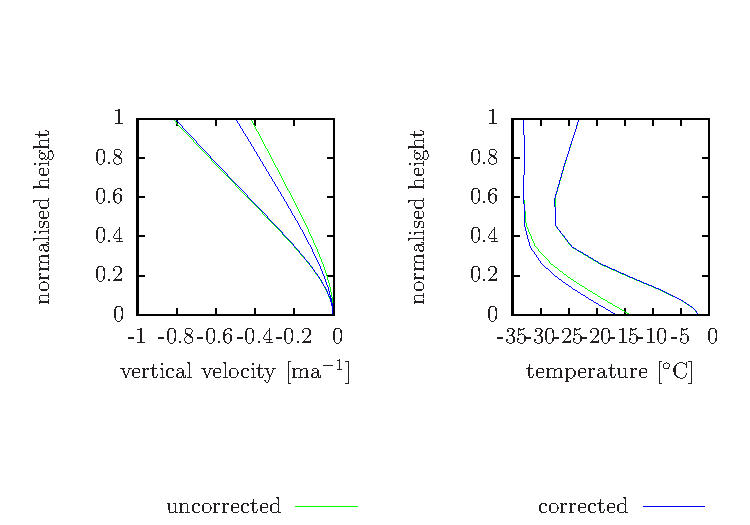
\includegraphics{\dir/gnu/wt_sigma.eps}
  \caption{Vertical velocity and temperature distribution for columns at the ice divide and a point half--way between the divide and the domain margin.}
  \label{kin.fig.wt_sigma}
\end{figure}
